\documentclass{article}

\usepackage{amsmath,amssymb}
\usepackage{tikz}
\usepackage{pgfplots}
\usepackage{xcolor}
\usepackage[left=2.1cm,right=3.1cm,bottom=3cm,footskip=0.75cm,headsep=0.5cm]{geometry}
\usepackage{enumerate}
\usepackage{enumitem}
\usepackage{marvosym}
\usepackage{tabularx}

\usepackage{listings}
\definecolor{lightlightgray}{rgb}{0.95,0.95,0.95}
\definecolor{lila}{rgb}{0.8,0,0.8}
\definecolor{mygray}{rgb}{0.5,0.5,0.5}
\definecolor{mygreen}{rgb}{0,0.8,0.26}
\lstdefinestyle{java} {language=java}
\lstset{language=java,
	basicstyle=\ttfamily,
	keywordstyle=\color{lila},
	commentstyle=\color{lightgray},
	stringstyle=\color{mygreen}\ttfamily,
	backgroundcolor=\color{white},
	showstringspaces=false,
	numbers=left,
	numbersep=10pt,
	numberstyle=\color{mygray}\ttfamily,
	identifierstyle=\color{blue},
	xleftmargin=.1\textwidth, 
	%xrightmargin=.1\textwidth,
	escapechar=§,
}

\usepackage[utf8]{inputenc}

\renewcommand*{\arraystretch}{1.4}

\newcolumntype{L}[1]{>{\raggedright\arraybackslash}p{#1}}
\newcolumntype{R}[1]{>{\raggedleft\arraybackslash}p{#1}}
\newcolumntype{C}[1]{>{\centering\let\newline\\\arraybackslash\hspace{0pt}}m{#1}}

\newcommand{\E}{\mathbb{E}}
\DeclareMathOperator{\rk}{rk}
\DeclareMathOperator{\Var}{Var}
\DeclareMathOperator{\Cov}{Cov}

\title{\textbf{Rechnernetze, Übung 4}}
\author{\textsc{Henry Haustein}}
\date{}

\begin{document}
	\maketitle
	
	\section*{Aufgabe 1}
	\begin{enumerate}[label=(\alph*)]
		\item Graph
		\begin{center}
			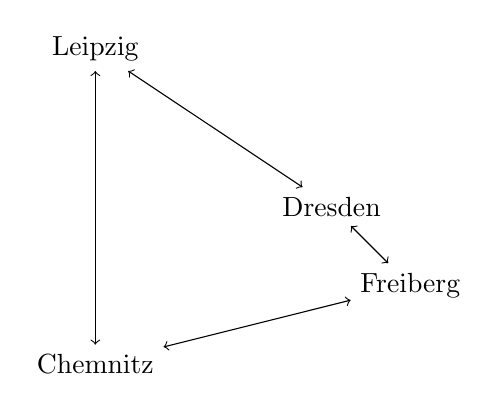
\begin{tikzpicture}
				\node at (0,0) (d) {Dresden};
				\node at (-3,2) (l) {Leipzig};
				\node at (-3,-2) (c) {Chemnitz};
				\node at (1,-1) (f) {Freiberg};
				
				\draw[<->] (d) -- (l);
				\draw[<->] (l) -- (c);
				\draw[<->] (c) -- (f);
				\draw[<->] (f) -- (d);
			\end{tikzpicture}
		\end{center}
		\item In der ersten Zeiteinheit können folgende Übertragungen stattfinden: : D $\to$ L, C $\to$ L, L $\to$ C, F $\to$ D und D $\to$ C. Die Verbindung C $\to$ D kann noch nicht stattfinden, da diese Verbindung entweder über Leipzig oder über Freiberg geht und keine Route frei ist. In der zweiten Zeiteinheit kann dann die Verbindung C $\to$ D aufgebaut werden, die insgesamt 2 Zeiteinheiten dauert. Insgesamt sind also 3 Zeiteinheiten notwendig.
		\item In der ersten Zeiteinheit können folgende Übertragungen stattfinden: : D $\to$ L, C $\to$ L, L $\to$ C, F $\to$ D und D $\to$ C. Die Verbindung C $\to$ D kann noch nicht stattfinden, da die Route über Leipzig nicht frei ist. In der zweiten Zeiteinheit findet die Verbindung dann aber statt, so dass insgesamt wieder 3 Zeiteinheiten gebraucht werden.
	\end{enumerate}

	\section*{Aufgabe 2}
	\begin{enumerate}[label=(\alph*)]
		\item Graph
		\begin{center}
			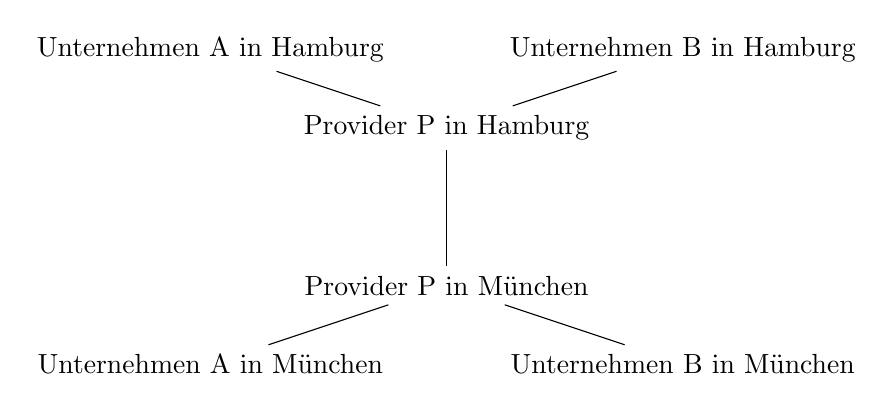
\begin{tikzpicture}
				\node at (0,0) (p1) {Provider P in Hamburg};
				\node at (0,-2) (p2) {Provider P in München};
				\node at (-3,1) (a1) {Unternehmen A in Hamburg};
				\node at (3,1) (b1) {Unternehmen B in Hamburg};
				\node at (-3,-3) (a2) {Unternehmen A in München};
				\node at (3,-3) (b2) {Unternehmen B in München};
				
				\draw (a1) -- (p1) -- (b1);
				\draw (p1) -- (p2);
				\draw (a2) -- (p2) -- (b2);
			\end{tikzpicture}
		\end{center}
		\item Da die Pakete mit der VLAN-ID 5 getagged werden, kann die MAC-Adresse eines Computers im konkurrierenden Unternehmen manipuliert werden, sodass der Provider die Daten an die Konkurrenz weiterleitet.
		\item Die Lösung ist eine Schachtelung der VLAN-IDs: Unternehmen A bekommt die VLAN-ID 1 und baut damit sein eigenes VLAN im Netz des Providers auf, genau so wie Unternehmen B die VLAN-ID 2 bekommt. So ist eine falsche Weiterleitung der Daten ausgeschlossen.
		\item Vom Unternehmen A wird zwischen SRC und Length wird die VLAN-ID 5 mit Header eingeschleust, der Provider hängt dann davor noch die VLAN-ID 1 mit Header.
	\end{enumerate}

	\section*{Aufgabe 3}
	\begin{enumerate}[label=(\alph*)]
		\item Die Tabellen sind \\
		\begin{minipage}[t]{0.3\textwidth}
			\begin{center}
				San Francisco \\
				\begin{tabular}{c|c|c}
					\textbf{Ziel-IP} & \textbf{von} & \textbf{nach} \\
					\hline
					230.3.0.0/16 & (1,-)  & (2,100) \\
					134.5.0.0/16 & (1,-) & (3,200)
				\end{tabular}
			\end{center}
		\end{minipage}
		\begin{minipage}[t]{0.3\textwidth}
			\begin{center}
				Chicago \\
				\begin{tabular}{c|c}
					\textbf{von} & \textbf{nach} \\
					\hline
					(1,100) & (2,101)
				\end{tabular}
			\end{center}
		\end{minipage}
		\begin{minipage}[t]{0.3\textwidth}
			\begin{center}
				Houston \\
				\begin{tabular}{c|c}
					\textbf{von} & \textbf{nach} \\
					\hline
					(1,200) & (3,201)
				\end{tabular}
			\end{center}
		\end{minipage} \\
		\vspace{0.2cm} \\
		\begin{minipage}[t]{0.45\textwidth}
			\begin{center}
				Washington \\
				\begin{tabular}{c|c}
					\textbf{von} & \textbf{nach} \\
					\hline
					(1,201) & (3,202)
				\end{tabular}
			\end{center}
		\end{minipage}
		\begin{minipage}[t]{0.45\textwidth}
			\begin{center}
				New York \\
				\begin{tabular}{c|c|c}
					\textbf{Ziel-IP} & \textbf{von} & \textbf{nach} \\
					\hline
					$\ast$ & (1,101)  & (4,-) \\
					$\ast$ & (2,202) & (3,-)
				\end{tabular}
			\end{center}
		\end{minipage}
		\item Die Zieladresse ist auf jeder Teilstrecke gleich 134.5.20.217 und die Header sind: Berkley $\to$ San Francisco nicht vorhanden, San Francisco $\to$ Chicago  100, Chicago $\to$ New York 101, New York $\to$ NYSE nicht vorhanden.
		\item Die Tabellen sind \\
		\begin{minipage}[t]{0.3\textwidth}
			\begin{center}
				San Francisco \\
				\begin{tabular}{c|c|c}
					\textbf{Ziel-IP} & \textbf{von} & \textbf{nach} \\
					\hline
					230.3.0.0/16 & (1,-)  & (2,100) \\
					134.5.0.0/16 & (1,-) & (3,200) \\
					$\ast$ & (2,301) & (1,-) \\
					$\ast$ & (3,402) & (1,-)
				\end{tabular}
			\end{center}
		\end{minipage}
		\begin{minipage}[t]{0.3\textwidth}
			\begin{center}
				Chicago \\
				\begin{tabular}{c|c}
					\textbf{von} & \textbf{nach} \\
					\hline
					(1,100) & (2,101) \\
					(2,300) & (1,301)
				\end{tabular}
			\end{center}
		\end{minipage}
		\begin{minipage}[t]{0.3\textwidth}
			\begin{center}
				Houston \\
				\begin{tabular}{c|c}
					\textbf{von} & \textbf{nach} \\
					\hline
					(1,200) & (3,201) \\
					(3,401) & (1,402)
				\end{tabular}
			\end{center}
		\end{minipage} \\
		\vspace{0.2cm} \\
		\begin{minipage}[t]{0.45\textwidth}
			\begin{center}
				Washington \\
				\begin{tabular}{c|c}
					\textbf{von} & \textbf{nach} \\
					\hline
					(1,201) & (3,202) \\
					(3,400) & (1,401)
				\end{tabular}
			\end{center}
		\end{minipage}
		\begin{minipage}[t]{0.45\textwidth}
			\begin{center}
				New York \\
				\begin{tabular}{c|c|c}
					\textbf{Ziel-IP} & \textbf{von} & \textbf{nach} \\
					\hline
					$\ast$ & (1,101)  & (4,-) \\
					$\ast$ & (2,202) & (3,-) \\
					217.8.0.0/16 & (4,-) & (1,300) \\
					217.8.0.0/16 & (3,-) & (2,400)
				\end{tabular}
			\end{center}
		\end{minipage}
		\item Dafür müssen die Tabellen von San Francisco und New York aktualisiert werden \\
		\begin{minipage}[t]{0.45\textwidth}
			\begin{center}
				San Francisco \\
				\begin{tabular}{c|c|c}
					\textbf{Ziel-IP} & \textbf{von} & \textbf{nach} \\
					\hline
					134.5.42.0/24 & (1,-) & (2,100) \\
					217.8.42.0/24 & (2,301) & (1,-) \\
					230.3.0.0/16 & (1,-)  & (2,100) \\
					134.5.0.0/16 & (1,-) & (3,200) \\
					$\ast$ & (2,301) & (1,-) \\
					$\ast$ & (3,402) & (1,-)
				\end{tabular}
			\end{center}
		\end{minipage}
		\begin{minipage}[t]{0.45\textwidth}
			\begin{center}
				New York \\
				\begin{tabular}{c|c|c}
					\textbf{Ziel-IP} & \textbf{von} & \textbf{nach} \\
					\hline
					134.5.42.0/24 & (1,101) & (3,-) \\
					217.8.42.0/24 & (3,-) & (1,300) \\
					$\ast$ & (1,101)  & (4,-) \\
					$\ast$ & (2,202) & (3,-) \\
					217.8.0.0/16 & (4,-) & (1,300) \\
					217.8.0.0/16 & (3,-) & (2,400)
				\end{tabular}
			\end{center}
		\end{minipage}
	\end{enumerate}
	
\end{document}